%% Dokumentenklasse (Koma Script)
\documentclass[%
   %draft,     % Entwurfsstadium
   final,      % fertiges Dokument
%%%% --- Schriftgröße ---
   11pt,
%%%% --- Sprache ---
   english,
   ngerman,           % Letzte Sprache ist die Hauptsprache, andere muss erst ausgewählt werden.
%%%% === Seitengröße ===
   a4paper,
%%%% === Optionen für den Satzspiegel ===
   %BCOR5mm,         % Zusaetzlicher Rand auf der Innenseite (Bindekorrektur)
   %DIV11,           % Seitengroesse (siehe Koma Skript Dokumentation!)
   %DIVcalc,         % automatische Berechnung einer guten Zeilenlaenge
   1.1headlines,     % Zeilenanzahl der Kopfzeilen
   %headinclude,     % Kopf einbeziehen
   headinclude=false,      % Kopf nicht einbeziehen
   %footinclude,     % Fuss einbeziehen
   footinclude=false,      % Fuss nicht einbeziehen
   %mpinclude,       % Margin einbeziehen
   mpinclude=false,        % Margin nicht einbeziehen
   pagesize,         % Schreibt die Papiergroesse in die Datei.
                     % Wichtig fuer Konvertierungen
%%%% === Layout ===
   oneside,          % einseitiges Layout
   %twoside,         % Seitenraender für zweiseitiges Layout
   onecolumn,        % Einspaltig
   %twocolumn,       % Zweispaltig
   %openany,         % Kapitel beginnen auf jeder Seite
   openright,        % Kapitel beginnen immer auf der rechten Seite
                     % (macht nur bei 'twoside' Sinn)
   %cleardoubleplain,    % leere, linke Seite mit Seitenstil 'plain'
   %cleardoubleempty,    % leere, linke Seite mit Seitenstil 'empty'
   titlepage,        % Titel als einzelne Seite ('titlepage' Umgebung)
   %notitlepage,     % Titel in Seite integriert
%%%% --- Absatzeinzug ---
   %                 % Absatzabstand: Einzeilig,
   %parskip,         % Freiraum in letzter Zeile: 1em
   %parskip*,        % Freiraum in letzter Zeile: Viertel einer Zeile
   %parskip+,        % Freiraum in letzter Zeile: Drittel einer Zeile
   %parskip-,        % Freiraum in letzter Zeile: keine Vorkehrungen
   %                 % Absatzabstand: Halbzeilig
   %halfparskip,     % Freiraum in letzter Zeile: 1em
   %halfparskip*,    % Freiraum in letzter Zeile: Viertel einer Zeile
   %halfparskip+,    % Freiraum in letzter Zeile: Drittel einer Zeile
   parskip=half,      % Freiraum in letzter Zeile: keine Vorkehrungen
   %                 % Absatzabstand: keiner
   %parindent,       % Eingerückt (Standard)
%%%% --- Kolumnentitel ---
   headsepline,      % Linie unter Kolumnentitel
   %headnosepline,   % keine Linie unter Kolumnentitel
   %footsepline,     % Linie unter Fussnote
   %footnosepline,   % keine Linie unter Fussnote
%%%% --- Kapitel ---
   %chapterprefix,   % Ausgabe von 'Kapitel:'
   chapterprefix=false,
   version=first,  % keine Ausgabe von 'Kapitel:'
%%%% === Verzeichnisse (TOC, LOF, LOT, BIB) ===
   listof=totoc,      % Tabellen & Abbildungsverzeichnis ins TOC
   %idxtotoc,        % Index ins TOC
   bibliography=totoc,
   verson=first,         % Bibliographie ins TOC
   %bibtotocnumbered, % Bibliographie im TOC nummeriert
   %liststotocnumbered, % Alle Verzeichnisse im TOC nummeriert
   toc=graduated,        % eingereuckte Gliederung
   %tocleft,         % Tabellenartige TOC
   %listsindent,      % eingereuckte LOT, LOF
   %listsleft,       % Tabellenartige LOT, LOF
   %pointednumbers,  % Überschriftnummerierung mit Punkt, siehe DUDEN !
   %pointlessnumbers, % Überschriftnummerierung ohne Punkt, siehe DUDEN !
   %openbib,         % alternative Formatierung des Literaturverzeichnisses
%%%% === Matheformeln ===
   %leqno,           % Formelnummern links
   fleqn,            % Formeln werden linksbuendig angezeigt
]{scrbook}%     Klassen: scrartcl, scrreprt, scrbook
% -------------------------------------------------------------------------
\usepackage[utf8]{inputenc}
% -------------- Daten für die Titelseite --> diese müssen angepasst werden!
\newcommand*{\thedockind}{Seminararbeit}
\newcommand*{\thetitle}{Administration in SAP BW 7.0}
\newcommand*{\thesubtitle}{mit der Data Warehousing Workbench}
\newcommand*{\theauthor}{-}
\newcommand*{\thematriculationnumber}{-} % Matrikelnummer
\newcommand*{\thebirthday}{-} % Geburtstag
\newcommand*{\thedegree}{-}
\newcommand*{\themajor}{-} % Studiengang
\newcommand*{\thedate}{\today} % \today kann durch ein Datum erstetzt werden.
\newcommand*{\thebetreuer}{-}
\newcommand*{\thezweitbetreuer}{-}
% -------------- Ende Daten für die Titelseite

\newcommand*{\anm}{\textcolor{red}}


%%% Doc: ftp://tug.ctan.org/pub/tex-archive/macros/latex/required/babel/babel.pdf
% Languagesetting
\usepackage{babel}	% Sprache

\usepackage{textpos} 


\usepackage{fixltx2e}	% Verbessert einige Kernkompetenzen von LaTeX2e
\usepackage{ellipsis}	% Korrigiert den Wei�raum um Auslassungspunkte

\usepackage{placeins} 

\usepackage{ifpdf}
\ifpdf
\pdfinfo {
	/Author (\theauthor)
	/Title (\thetitle)
	/Subject ()
	/Keywords ()
%	/CreationDate (D:YYYYMMTTHHMMSS)
}
\fi



%%% Doc: www.cs.brown.edu/system/software/latex/doc/calc.pdf
% Calculation with LaTeX
\usepackage{calc}

%%% Doc: ftp://tug.ctan.org/pub/tex-archive/macros/latex/contrib/xcolor/xcolor.pdf
% Farben
% Incompatible: Do not load when using pstricks !
\usepackage[
	table % Load for using rowcolors command in tables
]{xcolor}

\usepackage{tikz}
\usetikzlibrary{% 
   arrows,% 
   calc,% 
   fit,% 
   patterns,% 
   plotmarks,% 
   shapes.geometric,% 
   shapes.misc,% 
   shapes.symbols,% 
   shapes.arrows,% 
   shapes.callouts,% 
   shapes.multipart,% 
   shapes.gates.logic.US,% 
   shapes.gates.logic.IEC,% 
   er,% 
   automata,% 
   backgrounds,% 
   chains,% 
   topaths,% 
   trees,% 
   petri,% 
   mindmap,% 
   matrix,% 
   calendar,% 
   folding,% 
   fadings,% 
   through,% 
   positioning,% 
   scopes,% 
   decorations.fractals,% 
   decorations.shapes,% 
   decorations.text,% 
   decorations.pathmorphing,% 
   decorations.pathreplacing,% 
   decorations.footprints,% 
   decorations.markings,% 
   shadows} 
   
%%% Doc: ftp://tug.ctan.org/pub/tex-archive/macros/latex/required/graphics/grfguide.pdf
% Bilder
\usepackage[%
	%final,
	%draft % do not include images (faster)
]{graphicx}


% bessere Abstaende innerhalb der Tabelle (Layout))
% -------------------------------------------------
%%% Doc: ftp://tug.ctan.org/pub/tex-archive/macros/latex/contrib/booktabs/booktabs.pdf
\usepackage{booktabs}


%%% Doc: ftp://tug.ctan.org/pub/tex-archive/macros/latex/contrib/enumitem/enumitem.pdf
% Better than 'paralist' and 'enumerate' because it uses a keyvalue interface!
% Do not load together with enumerate.
%\usepackage{enumitem}

\usepackage{paralist}


%%% Doc: http://www.ctan.org/tex-archive/macros/latex/contrib/acronym/acronym.pdf
% Usage:
%        Definition: \acro{ acronym }[ short name ]{ full name }
%        Nutzung im Text: \ac{acronym}
 \usepackage[
 	footnote,	% Full names appear in the footnote
 	%smaller,		% Print acronym in smaller fontsize
 	%printonlyused %
 ]{acronym}
%\chapter*{Abkürzungsverzeichnis}
\begin{acronym}[BiPRO ] %Längster Begriff
\setlength{\itemsep}{-\parsep}
    \acro{LBG}{Location-based Game}
    \acro{UX}{User Experience}
    \acro{MMORPG} {Massively Multiplayer Online Role-Playing Game}
    \acro{EA}{Electronic Arts}
	\acro{GAAP}{Generally accepted accounting principles}
\end{acronym}



%% Kopf und Fusszeilen====================================================
%%% Doc: ftp://tug.ctan.org/pub/tex-archive/macros/latex/contrib/koma-script/scrguide.pdf
\usepackage[%
   automark,         % automatische Aktualisierung der Kolumnentitel
   %nouppercase,      % Grossbuchstaben verhindern
   %markuppercase    % Grossbuchstaben erzwingen
   %markusedcase     % vordefinierten Stil beibehalten
   %komastyle,       % Stil von Koma Script
   %standardstyle,   % Stil der Standardklassen
]{scrpage2}



%% UeberSchriften (Chapter und Sections) =================================
% -- Ueberschriften komlett Umdefinieren --
%%% Doc: ftp://tug.ctan.org/pub/tex-archive/macros/latex/contrib/titlesec/titlesec.pdf
\usepackage{titlesec}

% -- Section Aussehen veraendern --
% --------------------------------
%% -> Section mit Unterstrich
% \titleformat{\section}
%   [hang]%[frame]display
%   {\usekomafont{sectioning}\Large}
%  {\thesection}
%   {6pt}
%   {}
%   [\titlerule \vspace{0.5\baselineskip}]
% --------------------------------

% -- Chapter Aussehen veraendern --
% --------------------------------
\titleformat{\chapter}[block]	% {command}[shape]
  {\usekomafont{chapter}\huge\sffamily\bfseries}	% format
  {   										% label
      {\thechapter.} \filright%
  }%}
  {1pt}										% sep (from chapternumber)
  {\vspace{0.5pc} \filright {}}   % {before}[after] (before chaptertitle and after)
  [\vspace{0.5pc} \filright {}]

% \titleformat{\chapter}[]%
%    {\usekomafont{chapter}\huge\sffamily\bfseries}%
%    {\thechapter}%
%    {1em}%
%    {}%


\usepackage{rotating}


\usepackage[numbers,square]{natbib}
%\usepackage{cite}
%\bibliographystyle{dinat}
%\citestyle{alpha}
\bibliographystyle{alphadin}


% Quotes =================================================================
%% Doc: ftp://tug.ctan.org/pub/tex-archive/macros/latex/contrib/csquotes/csquotes.pdf
% Advanced features for clever quotations
\usepackage[%
   babel,            % the style of all quotation marks will be adapted
                     % to the document language as chosen by 'babel'
   german=quotes,		% Styles of quotes in each language
   %german=guillemets,
   english=british,
   french=guillemets
]{csquotes}
\usepackage{floatflt}

\usepackage{wrapfig}

%\usepackage{subfigure}

\usepackage{blindtext}

\usepackage{listings}
\lstset{language=html}
\definecolor{lila}{RGB}{112, 6, 147}
\definecolor{kommentgreen}{RGB}{5,132,71}
\definecolor{grey}{RGB}{242,242,242}  
\definecolor{darkgreen}{named}{green}
\definecolor{darkblue}{named}{blue}
\definecolor{lightblue}{RGB} {63,95,191}
\definecolor{darkred}{named}{red}
\definecolor{grau}{named}{gray}
\definecolor{fh_orange}{rgb}{0.953,0.201,0}
\definecolor{fh_grau}{rgb}{0.76,0.75,0.76}
\definecolor{light_green}{RGB}{199,199,199}

\definecolor{listinggray}{gray}{0.9}
\definecolor{lbcolor}{rgb}{0.9,0.9,0.9}

\lstset{
	tabsize=3,
	float=tbph,
	frame=single,
	extendedchars,
	breaklines=true,
	basicstyle=\fontsize{9pt}{9pt}\selectfont,
	columns=flexible, %ist notwendig, damit man Quelltext aus den Listings kopieren kann
	numbers=left, 
	numberstyle=\color{black},
	captionpos=b,
	aboveskip=7mm,
	backgroundcolor=\color{grey}
}

\lstdefinestyle{java}
{
	language=Java,
	keywordstyle=\color{lila},  	% underlined bold black keywords 
	identifierstyle=\color{blue}, 
	commentstyle=\color{kommentgreen}, % white comments 
	stringstyle=\color{black},
}

\lstdefinestyle{xml}
{
	language=xml,
	basicstyle=\fontsize{9pt}{9pt}\selectfont\color{black},
	keywordstyle=\color{lila},  	% underlined bold black keywords 
	%Hier können bei Bedarf noch weitere Keywords eingetragen werden
	keywords={name, value, version, encoding, id, type, xmlns:xsi, ref, namespace,bachelorarbeit,thema,vorname,note},
	identifierstyle=\color{black},  
	stringstyle=\color{blue},  
	commentstyle=\color{lightblue},
	morecomment=[s]{<!--}{-->},
	rulecolor=\color{black}
}


\colorlet{punct}{red!60!black}
\definecolor{background}{HTML}{EEEEEE}
\definecolor{delim}{RGB}{20,105,176}
\colorlet{numb}{magenta!60!black}



\lstdefinelanguage{json}{
    basicstyle=\fontsize{9pt}{9pt}\selectfont\color{black},
    literate=
     *{0}{{{\color{numb}0}}}{1}
      {1}{{{\color{black}1}}}{1}
      {2}{{{\color{numb}2}}}{1}
      {3}{{{\color{black}3}}}{1}
      {4}{{{\color{numb}4}}}{1}
      {5}{{{\color{numb}5}}}{1}
      {6}{{{\color{numb}6}}}{1}
      {7}{{{\color{numb}7}}}{1}
      {8}{{{\color{numb}8}}}{1}
      {9}{{{\color{numb}9}}}{1}
      {:}{{{\color{punct}{:}}}}{1}
      {,}{{{\color{punct}{,}}}}{1}
      {[}{{{\color{delim}{[}}}}{1}
      {]}{{{\color{delim}{]}}}}{1},
      keywordstyle=\color{lila},  	% underlined bold black keywords 
	%Hier können bei Bedarf noch weitere Keywords eingetragen werden
	keywords={name, value, version, encoding, id, type, xmlns:xsi, ref, namespace,bachelorarbeit,thema,vorname,note,},
}


% Taken from Lena Herrmann at 
% http://lenaherrmann.net/2010/05/20/javascript-syntax-highlighting-in-the-latex-listings-package
%\documentclass{article}
%\usepackage{listings}
%\usepackage{color}
\definecolor{lightgray}{rgb}{.9,.9,.9}
\definecolor{darkgray}{rgb}{.4,.4,.4}
\definecolor{purple}{rgb}{0.65, 0.12, 0.82}

\lstdefinelanguage{JavaScript}{
  keywords={typeof, new, true, false, catch, function, return, null, catch, switch, var, if, in, while, do, else, case, break},
  keywordstyle=\color{blue}\bfseries,
  ndkeywords={class, export, boolean, throw, implements, import, this},
  ndkeywordstyle=\color{darkgray}\bfseries,
  identifierstyle=\color{black},
  sensitive=false,
  comment=[l]{//},
  morecomment=[s]{/*}{*/},
  commentstyle=\color{purple}\ttfamily,
  stringstyle=\color{red}\ttfamily,
  morestring=[b]',
  morestring=[b]"
}

\lstset{
   language=JavaScript,
   backgroundcolor=\color{lightgray},
   extendedchars=true,
   basicstyle=\footnotesize\ttfamily,
   showstringspaces=false,
   showspaces=false,
   numbers=left,
   numberstyle=\footnotesize,
   numbersep=9pt,
   tabsize=2,
   breaklines=true,
   showtabs=false,
   captionpos=b
}

\lstset{literate=%
{Ö}{{\"O}}1
{Ä}{{\"A}}1
{Ü}{{\"U}}1
{ß}{{\ss}}2
{ü}{{\"u}}1
{ä}{{\"a}}1
{ö}{{\"o}}1
}


\usepackage{multicol}

\usepackage{nameref}

\usepackage{tabularx}

\usepackage{subfigure}

\usepackage{hyperref}
\hypersetup{breaklinks=true}
\hypersetup{colorlinks=true,linkcolor=black,urlcolor=black,citecolor=black}
%\hypersetup{frenchlinks}	% Use small caps instead of color for links
%\hypersetup{pdfpagemode=FullScreen}
%\hypersetup{pdfstartpage=3}
%\hypersetup{pdfstartview=Fit}


% Tabellen ueber mehere Seiten
% ----------------------------
%%% Doc: ftp://tug.ctan.org/pub/tex-archive/macros/latex/contrib/carlisle/ltxtable.pdf
% \usepackage{ltxtable} % Longtable + tabularx
                        % (multi-page tables) + (auto-sized columns in a fixed width table)
% -> nach hyperref laden
%\usepackage{ltxtable}
%\usepackage{longtable}
\usepackage{tabulary}


% Schusterjunge und Hurenkinder verhindern
\clubpenalty=1000
\widowpenalty=1000
\displaywidowpenalty=1000

% Trennen von Bindestrich oder so ...
%\defaulthyphenchar=127

\usepackage[T1]{fontenc}
\usepackage{alltt}
\usepackage{marvosym}
\usepackage{fancybox}
\usepackage[hang,small,bf]{caption}
\usepackage{float} 
\usepackage{multirow}
\usepackage{pgfplots}
\usepackage{tikz}
\usepackage{pdfpages} 
\addtokomafont{caption}{\sffamily\small}
\setkomafont{captionlabel}{\sffamily\small}

\newcommand{\keyword}[1]{\textbf{#1}}
%\newcommand{\filename}[1]{\texttt{#1}}
\newcommand{\inlinecode}[1]{\lstinline!#1!}


% Umbenennung von "Listings"
\addto\captionsngerman{%
  \renewcommand{\lstlistlistingname}{Quelltextverzeichnis}%
  \renewcommand{\lstlistingname}{Quelltext}%
  \renewcommand{\}}{}
}

\usepackage{blindtext}
\usepackage{helvet}	%Paket für die Schriftart

\renewcommand{\familydefault}{\sfdefault}	%sorgt für einheitliche Schriftart im gesamten Dokument
\setcounter{secnumdepth}{2} %legt die Ebene fest, bis zu der nummeriert wird
\setcounter{tocdepth}{2} %legt fest wieviele Ebenen im Inhaltsverzeichnis vorkommen


\begin{document}

	%\captionsetup[figure]{singlelinecheck=false} %sorgt für eine Linksbündige Bildunterschrift
	%\captionsetup[lstlisting]{singlelinecheck=off}
	\captionsetup{singlelinecheck=off}
	
  \sffamily		% Schriftart Serifenlos wählen
  \linespread {1.25}\selectfont %Zeilenabstand: 1.25 da er von Haus aus 1.2 ist und 1,25 * 1,2 = 1,5

	%Titelseite einfügen
	
\begin{titlepage}
		
%%%%%%%%%%%%%%%%%%%%%%%%%%%%%% -*- Mode: Latex -*- %%%%%%%%%%%%%%%%%%%%%%%%%%%%
%% 
%% pa_ba_titelblatt.tex 
%% 
%% Copyright (C) 2008 Alexander Sprack / Claudia Holz
%% 
%%%%%%%%%%%%%%%%%%%%%%%%%%%%%%%%%%%%%%%%%%%%%%%%%%%%%%%%%%%%%%%%%%%%%%%%%%%%%%%
  \begin{textblock}{6.5}(-1,-3)
    \begin{color}{light_green}
      \rule{6.8cm}{33cm}    
    \end{color}
  \end{textblock}
  \begin{textblock}{6.5}(-1.2,-0.7)
%  \includegraphics[width=3.8cm]{my-fh-logo}% selbst basteln, falls gewünscht! 
                                            % Das offizielle Logo ist nicht
                                            % gestattet!! Bitte BEACHTEN!!!
  \end{textblock}
  \begin{textblock}{6.5}(-0.8,1)
    {\Large \textsf{\thedockind}}            
  \end{textblock}

  \begin{textblock}{8}(4.5,2)
    {\noindent \huge 
      \textsf{\textbf{\thetitle\\[0.3cm] 
          \Large  \thesubtitle\\[0.05cm]
          }} }
  \end{textblock}


  \begin{textblock}{6}(4.5,6.5)\noindent
    \textsf{An der Fachhochschule Dortmund\\
    im Fachbereich Informatik\\
    Studiengang \themajor \\
    erstellte \thedockind \\
    Noch mehr Text? :) \\
    \thedegree}
  \end{textblock}

  \begin{textblock}{6.5}(-0.4,10.0)
    \noindent
    \textsf{von \\
      \theauthor \\
      geb.\ am \thebirthday  \\
      Matr.-Nr. \thematriculationnumber\\[0.7cm]
      Betreuer:\\
       \noindent\hspace*{6mm} \thebetreuer \\
       \noindent\hspace*{6mm} \thezweitbetreuer\\ [0.5cm]
      Dortmund, \today}    
  \end{textblock}
	

\end{titlepage}



%\thispagestyle{empty}

	
	

	\frontmatter	
	        %römische Nummerierung für Inhaltsverzeichnis aktivieren
	
	%\chapter{Abstract} 
%\label{sec:}
Diese Arbeit gibt einen Einblick in den Entwicklungsprozess eines Location-based Games. Es wird der Hintergrund von Location-based games, kurz LBG, erläutert 
	
	\tableofcontents	    %Inhaltsverzeichnis erstellen
	\mainmatter	 		%Arabische Seitenummerierung

	\pagestyle{scrheadings}
	
	
	% ----------------- Einfügen des eigentlichen Textes
	


    \chapter{Einleitung}
\label{Kapitel:Einleitung}


\section{Überblick}
 
 Die Menge an analysierbaren  Informationen und den dazugehörigen Daten in Unternehmen nehmen immer stärker zu.  Durch den Zuwachs an Daten wird es aber auch immer schwieriger diese effektiv auszuwerten. Die  Daten in einzelnen und unterschiedlichen Programmen zu verwalten und zwischen diesen auszutauschen lässt sich zeitlich nicht mehr bewerkstelligen. Außerdem sind einige Datenquellen so stark angewachsen, das sie sich mit herkömmlichen Tabellenkalkulationsprogrammen nicht mehr auswerten lassen.
 
 
Es wird ein Umfeld bzw. System benötigt, welches diesen Ansprüchen gerecht wird. Ein Business Intelligence Umfeld mit einem zentralen Data Warehouse kann vielen dieser Anforderungen mehr als gerecht werden. Die neu aufgestellte Datenbasis steht dem gesamten Unternehmen zur Verfügung und führt so zu einer Vereinheitlichung der Datenstrukturen sowie deren Semantik. Eine funktionierende Business Intelligence erlaubt dem Unternehmen in kürzester Zeit, hochaktuelle Informationen und dynamische Berichte zu generieren, um flexibel am Markt agieren zu können. Komplexe Data Mining Anwendungen finden Muster in den Daten, um Geschäftsprozesse zu optimieren, die verborgenen Wünsche des Kunden aufzudecken oder völlig neue Geschäftsmodelle zu entwickeln.
 
Ziel dieser Arbeit ist es, einen fundierten Überblick über die Bedeutung der Business Intelligence, des Data Warehouse sowie dem Reporting in diesem Umfeld zu geben und am Ende mögliche Umsetzungsmöglichkeiten zu demonstrieren.
 
\section{ Aufbau der Arbeit}
 
Im zweiten Kapitel wird der Frage nachgegangen, was man überhaupt unter dem Begriff „Business Intelligence“ versteht und ob es eine Möglichkeit gibt, diesen genau zu definieren. Hierfür wird ein kurzer Überblick über die geschichtliche Entwicklung der Informationssysteme innerhalb der Unternehmen eingeschoben, der schließlich in einem Referenzmodell mündet. Dieses Modell zeigt, wie aktuelle BI-Landschaften aussehen könnten. Hier wird versucht zu erklären, wie ein Business Intelligence System funktioniert und welche Möglichkeiten man hat, dieses effektiv zu nutzen.
 
Das Konzept und die Funktionsweise eines Data Warehouse hat, aufbauend auf dem zweiten Kapitel, das dritte Kapitel zum Inhalt. Es versucht das allgemein anerkannte Data Warehouse Konzept und die darauf aufbauende Referenzarchitektur darzustellen und die Prozesse innerhalb des Data Warehouse entsprechend zu erläutern. Hierfür wird aufgeführt, welche Anforderungen an die Systeme zu stellen sind um dem analytischen Gedanken zu folgen. Das Kapitel wird mit einer Einführung in die multidimensionalen Datenmodelle und deren Abbildung im relationalen Umfeld abgeschlossen.
 
Kapitel 4 stellt die Erfordernisse eines Reportings dar und versucht die Thematiken Business Intelligence und Data Warehouse in dieses Thema zu integrieren. Es soll aufzeigen, wie sich die gewonnenen Erkenntnisse der vorherigen Kapitel schließlich auch im Bereich des Unternehmensreportings widerspiegeln. Hierzu orientiert sich das Kapitel an der Management Reporting Excellence, der Idealform des Management Reportings.
 
Abschließend soll das fünfte Kapitel aufzeigen, wie man mit Open Source Produkten ein Business Intelligence Umfeld aufbauen und administrieren kann. Es stellte sich heraus, dass es hier zu einigen Problemen kommen kann, die ebenfalls im Kapitel erläutert werden.
 
Die Arbeit endet mit einer Schlussbetrachtung, die abschließend aufzeigen soll, ob die Problemstellungen der einzelnen Kapitel gelöst worden sind und welche Fragen eventuell nicht beantwortet werden konnten.



\chapter{Begriffserläuterung}
\begin{description}
	\item [Data Warehouse bzw. Business Warehouse] ist eine von den operativen Datenverarbeitungssystemen separierte Datenbank, auf die nur Lesezugriff besteht. In regelmäßigen Abständen werden aus den operativen DV-Systemen unternehmensspezifische, historische und daher unveränderliche Daten zusammengetragen, vereinheitlicht, nach Nutzungszusammenhängen geordnet, verdichtet und dauerhaft in der Datenbasis des Data Warehouses archiviert. Ziel ist die Verbesserung der unternehmensinternen Informationsversorgung (Wissensmanagement) und damit der Unterstützung strategischer Entscheidungen. Als analytisches System liefert es Informationen zur Problemanalyse - Online Analytical Processing (OLAP) -, die durch die Anwendung von Methoden (z.B. des Data Mining) generiert werden.  \href{http://wirtschaftslexikon.gabler.de/Definition/data-warehouse.html?referenceKeywordName=Business+Warehouse}{\textbf{QUELLE}}
\end{description}




Was ist Buisness Warehouse und Data Warehouse kurze Definition \\
Ein Data Warehouse ist kein Produkt, sondern ein Konzept, das sich der Datenproblematik von managementunterstuetzenden Systemen annimmt\\
A data warehouse is a subject-oriented, integrated, nonvolatile, time-variant collection of data in support of management’s decision \\

1. subject-oriented: Die Themenausrichtung an Sachverhalten des Unternehmens, z.B. Kunden- oder Produktkriterien, wird im BW durch das konsequente Einordnen aller Daten in Fachbereiche und durch die Bezugnahme auf Geschäftsprozesse realisiert (Seemann/Schmalzridt/Lehmann 2001, 18). Im Gegensatz dazu sind operative Daten immer auf einzelne betriebliche Funktionen bezogen (Schinzer/Bange/Mertens 1999, 14 - Bange/ Schinzer o.J., 1). \\
2. integrated: Mit dem DW-Konzept wird eine unternehmensweite Integration von Daten in einem einheitlich gestalteten System angestrebt (Mucksch/Behme 2000, 11). Verein- heitlichung und Integration externer und interner Daten bedeutet weniger die physische Zentralisierung der Daten in einem einzigen Datenpool, sondern deren logische Ver- bindung. Integration bedeutet konsistente Datenhaltung im Sinne einer Struktur- und Formatvereinheitlichung durch Maßnahmen wie Vergabe eindeutiger Bezeichnungen, Anpassung der Datenformate und Herstellung einer semantischen Integrität (Mucksch/ Behme 2000, 11ff.). Ebenso tragen Elemente wie einheitliche Merkmale und standardi- sierte Kennzahlen zu einer Datenintegration bei.\\
3. nonvolatile: Bei einem DW handelt es sich um eine dauerhafte Sammlung von Informationen, auf die im Gegensatz zu OLTP-Systemen (online transaction processing3) nur in Form von Lese- und Einfügeoperationen zugegriffen werden darf, um die Nicht- Volatilität der Daten sicherzustellen.4 Dieser Forderung kann jedoch nur bedingt zuge- stimmt werden, da Korrekturen von aus Quellsystemen geladenen Daten auf jeden Fall möglich sein müssen (Behme 1996, 31). Das BW bietet hierfür eine Eingangsablage in Form der Persistent Staging Area (PSA)5, in der manuelle Korrekturen zur Validierung und Fehlerbehebung nach dem Extraktionsvorgang durchgeführt werden können (SAP 2000a, 1; SAP 2000b).\\
4. time-variant: Während bei operativen Systemen eine zeitpunktgenaue Betrachtung der Daten im Mittelpunkt steht, liegt das Interesse bei Auswertungen im DW eher in einer Zeitraumbetrachtung, z.B. einer Trendanalyse (Behme 1996, 31). Der Zeitraumbezug ist daher impliziter oder expliziter Bestandteil der Daten in einem DW. Ein Ansatz zur Herstellung dieses Zeitraumbezugs im BW ist die obligatorische Verwendung einer Zeitdimension in jedem Informationsspeicher.


\begin{figure}[H]
    \centering
    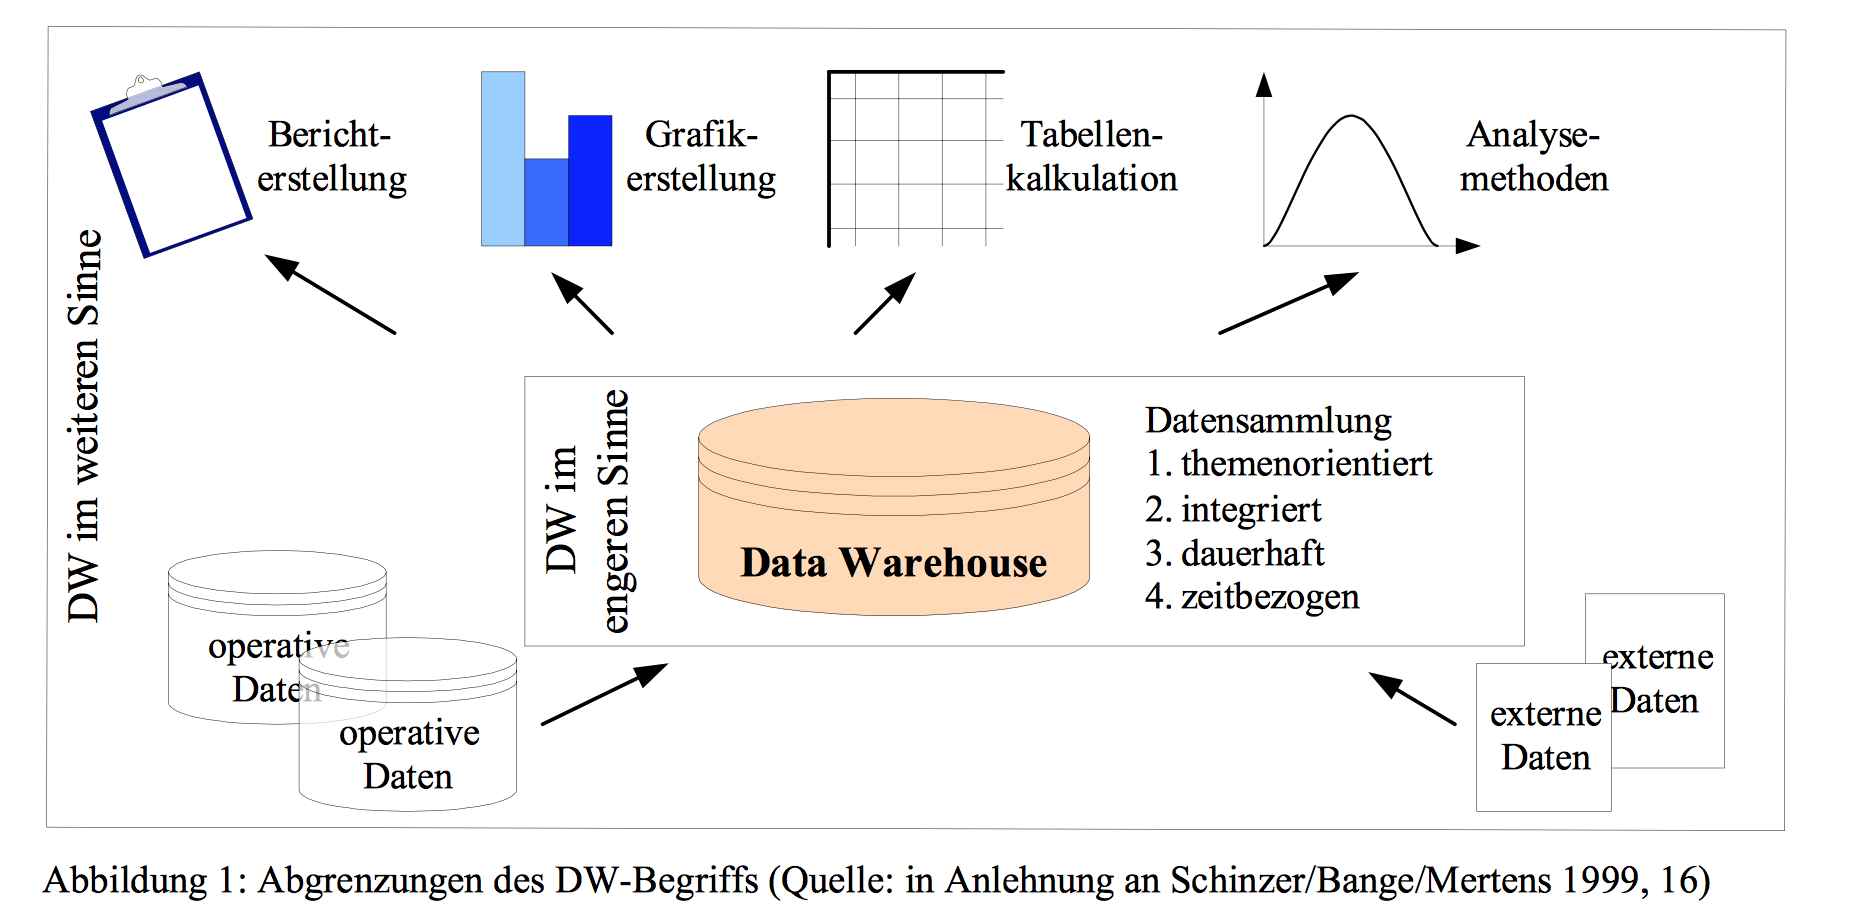
\includegraphics[width=1\textwidth]{files/DWOverview}
    \caption{Abgrenzungen des DW-Begriffs Q:(Schinzer/Bange/Mertens 1999, S.16)}
    \label{pic:DWOverview}
\end{figure}




Text

    \chapter{Die Data Warehousing Workbench}
\label{Abschnitt:Motivation}

\begin{figure}[H]
    \centering
    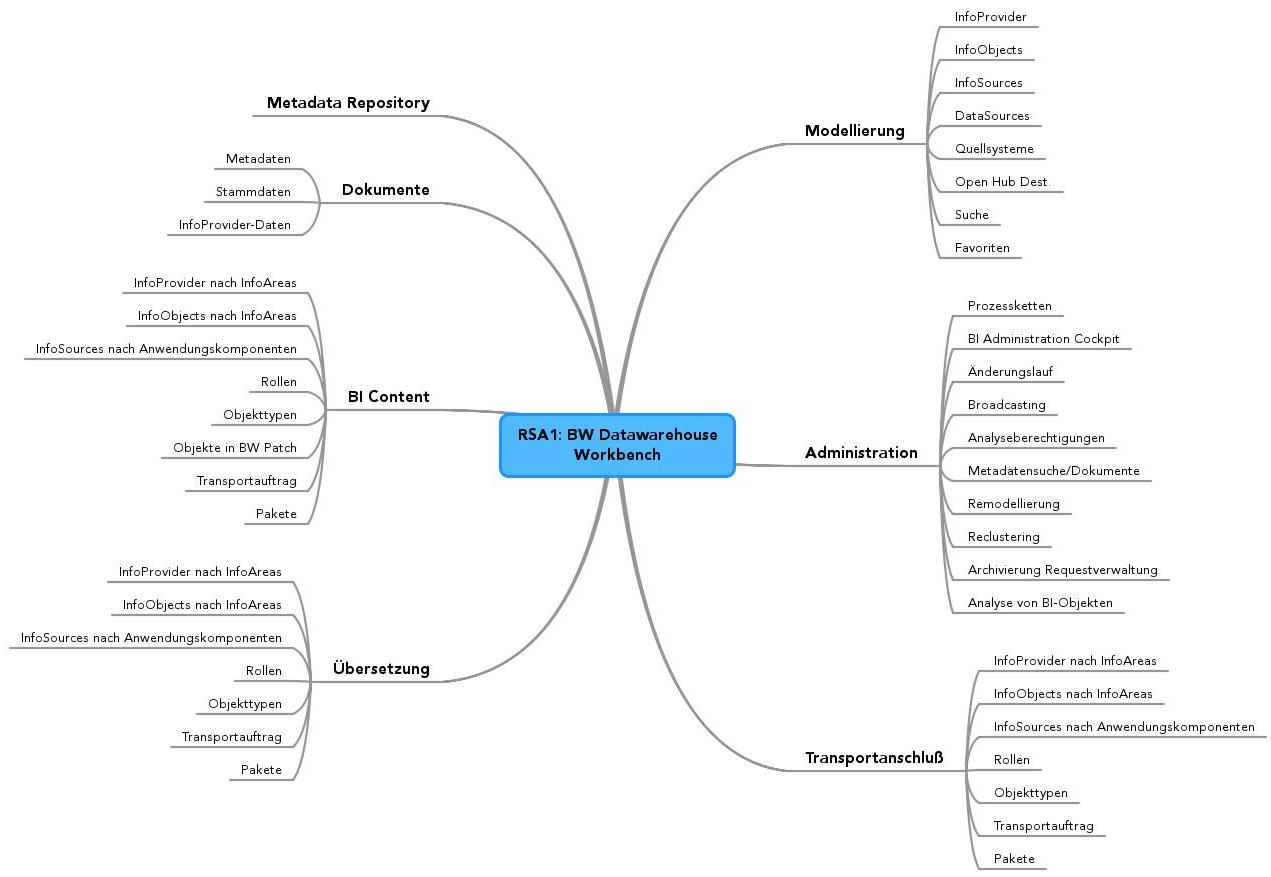
\includegraphics[width=1\textwidth]{files/RSA1Mindmap}
    \caption{Übersicht über RSA1}
    \label{pic:RSA1}
\end{figure}


Die \textit{ Data Warehousing Workbench} lässt sich in die folgenden sieben Module unterteilen, welche in \textbf{Abb. \ref{pic:RSA1}} in einem übersichtlichen Diagramm aufgelistet sind.\\

\begin{description}
\item[Modellierung:] Dieses Modul dient zur Modellierung von Daten und es werden verschiedene BI-Objekte bereitgestellt, welche zur Integration, Transformation, Konsolidierung, Bereinigung und Ablage von Daten genutzt werden können. Die verfügbaren BI-Objekte sind folgende:
\begin{itemize}
\item \textbf{InfoProvider:}
Oberbegriff für BI-Objekte, in die Daten hinein geladen werden können, bzw. Sichten auf die bereits geladenen Daten darstellen. Diese Daten können zu einem späteren Zeitpunkt mit dem BEx Query-Designer ausgewertet werden.

BI-Objekte sind zum einen Objekte, in denen Daten physisch vorhanden sind, wie InfoCubes, DataStore-Objekte und InfoObjects (Merkmale mit Attributen oder Texten). Zum anderen zählen dazu auch Objekte, die keine physische Datenablage darstellen, wie InfoSets, VirtualProvider und MultiProvider.

\item \textbf{InfoCubes:}
Spezifischere Variante eines InfoProviders.
Ein InfoCube beschreibt einen in sich geschlossenen Datenbestand z.B. eines betriebswirtschaftlichen Bereichs. Dieser Datenbestand kann mit dem BEx Query-Designer ausgewertet werden.

Ein InfoCube besteht aus relationalen Tabellen, die nach dem Sternschema zusammengestellt sind: eine große Faktentabelle im Zentrum und mehrere sie umgebende Dimensionstabellen.
Sie werden aus InfoSources oder anderen InfoProvidern mit Daten versorgt und stehen im Anschluss für das Reporting bzw. die Analyse zur Verfügung.

\item \textbf{InfoSources}
Es wird zwischen zwei Arten von InfoSources unterschieden:
-InfoSources mit \textit{flexibler} Fortschreibung
-InfoSources mit \textit{direkter} Fortschreibung

Diese bestehen aus einer Menge von Informationen, die zusammengefasst und bereitgestellt werden. Diese Informationen können Bewegungsdaten und Stammdaten sein.

Beide Arten transformieren die geladenen Daten durch Übertragungsregeln, die vorher definiert werden müssen. Die Regeln beziehen sich auf die Kombination von einer InfoSource und einem Quellsystem bzw. auf jedes InfoObjekt. Eine InfoSource kann mehrere InfoProvider mit Daten beliefern und selbst von mehreren Quellsystemen mit Daten versorgt werden.
Bei der flexiblen Fortschreibung werden die Daten in die Datenziele (InfoCube, DataStore-Objekt, Stammdaten) geladen.
Bei der direkten Fortschreibung können Stammdaten eines InfoObjects direkt in die Stammdatentabelle fortgeschrieben werden (dies ist nur mit Stammdaten möglich).

\end{itemize}
Die Grafische Oberfläche ist in  \textbf{Abb. \ref{pic:Modellierung}}  zu sehen.
\begin{figure}[H]
    \centering
    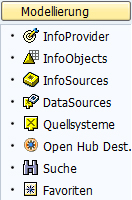
\includegraphics[width=0.2\textwidth]{files/Modellierung}
    \caption{Das Modellierungsmenü}
    \label{pic:Modellierung}
\end{figure}
\item[Administration:] Hier befindet sich eine Ansicht für die verschiedensten Prozessketten, sowie das BI Administration Cockpit. Jenes wird verwendet, um die Performance von BI-Systemen zu überwachen. Es liefert einen zentralen Einstiegspunkt, sowie ein real-Time Monitoring und verschiedene Laufzeitstatistiken. Es bietet Zugriff auf Berichte und Anwendungen, die den Anwender bei der Ermittlung und Analyse von Problemen unterstützt. Es können BI-Objekte nachverfolgt und die Performance von BI-Aktivitäten optimiert werden.
Die Grafische Oberfläche ist in  \textbf{Abb. \ref{pic:Administration}}  zu sehen.
\begin{figure}[H]
    \centering
    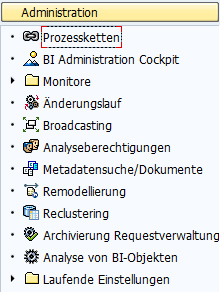
\includegraphics[width=0.4\textwidth]{files/Administration}
    \caption{Das Administrationsmenü}
    \label{pic:Administration}
\end{figure}
\item[BI Content:] Die Struktur der verarbeiteten Geschäftsinformationen eines Unternehmens kann zu Auswertungszwecken im BI Content modelliert werden. Diese Modelle setzen sich aus verschiedenen Metadaten-Objekttypen zusammen. Hierbei werden vorkonfigurierte zur Analyse betriebswirtschaftlicher Fragestellungen verwendet. Wichtig hierbei ist, dass die Erzeugung, Verwendung, Überarbeitung und der Transport der BI-Objekte konsistent gehalten wird. Ein enthaltenes Konzept ist das \textit{BI-Versionskonzept} und eine Hauptfunktionalität ist die Übernahme von neuem BI Content in das Produktivsystem.
Die Grafische Oberfläche ist in \textbf{Abb. \ref{pic:BIContent}} zu sehen.
\begin{figure}[H]
    \centering
    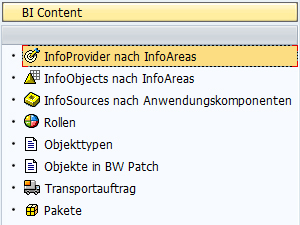
\includegraphics[width=0.45\textwidth]{files/BIContent}
    \caption{das BI Content Menü}
    \label{pic:BIContent}
\end{figure}
\item[Transportanschluss:] Hier werden die selben Funktionalitäten wie in dem Modul \textit{BI Content} unterstützt, es besteht allerdings noch zusätzlich die Möglichkeit, BI-Objekte im XML-Format zu importieren bzw. zu exportieren.
Die Grafische Oberfläche ist in \textbf{Abb. \ref{pic:Transportanschluss}} zu sehen.
\begin{figure}[H]
    \centering
    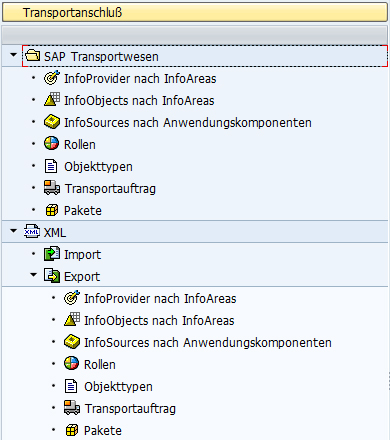
\includegraphics[width=0.55\textwidth]{files/Transportanschluss}
    \caption{Das Transportanschluss Menü}
    \label{pic:Transportanschluss}
\end{figure}
\item[Dokumente:] Zu jedem BI-Objekt können jeweils ein oder mehrere Dokumente in verschiedenen Formaten, Versionen und Sprachen hinzugefügt, verlinkt und durchsucht werden. Diese Dokumente sind in drei Klassen unterteilt und können jeweils \textit{Metadaten}, \textit{Stammdaten} oder \textit{InfoProvider-Daten} zugeordnet werden.
Die Grafische Oberfläche ist in  \textbf{Abb. \ref{pic:Dokumente}}  zu sehen.
\begin{figure}[H]
    \centering
    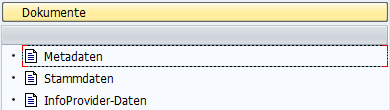
\includegraphics[width=0.6\textwidth]{files/Dokumente}
    \caption{Das Dokumente Menü}
    \label{pic:Dokumente}
\end{figure}
\item[Übersetzung:] Um eine Internationalisierung umsetzen zu können, können mit Hilfe des Moduls \textit{Übersetzung} die Kurz- und Langtexte von BI-Metadaten-Objekten vereinfacht übersetzt werden. Zusätzlich kann die Übersetzungsumgebung, die der SAP Web Application Server (ABAP) beinhalted, verwendet werden.
Die Grafische Oberfläche ist in \textbf{Abb. \ref{pic:Uebersetzung}} zu sehen.
\begin{figure}[H]
    \centering
    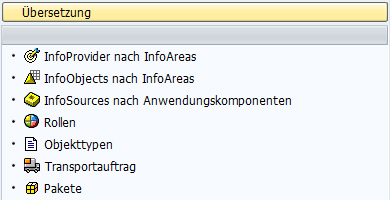
\includegraphics[width=0.6\textwidth]{files/Uebersetzung}
    \caption{Das Übersetzungsmenü}
    \label{pic:Uebersetzung}
\end{figure}
\item[Metadata Repository:] Das Metadata Repository basiert auf HTML und ermöglicht einen zentralen Zugriff auf Informationen von Metadaten-Objekten. Zu diesen Metadaten gehören zum Beispiel wichtige Eigenschaften der Objekte und die Verknüpfungen mit anderen Objekten.
\end{description}





    \chapter{Administration in der Workbench}
\label{Kapitel:Einleitung}
Text


\section{Unterkapitel}
\label{Abschnitt:Motivation}


Text

    \chapter{Fazit}
\label{Kapitel:Einleitung}
Text


\section{Unterkapitel}
\label{Abschnitt:Motivation}


Text

    

    
    
    
	% ----------------- Ende des eigentlichen Textes
	

	%Verzeichnisse erstellen
  %\chapter*{Abkürzungsverzeichnis}
\begin{acronym}[BiPRO ] %Längster Begriff
\setlength{\itemsep}{-\parsep}
    \acro{LBG}{Location-based Game}
    \acro{UX}{User Experience}
    \acro{MMORPG} {Massively Multiplayer Online Role-Playing Game}
    \acro{EA}{Electronic Arts}
	\acro{GAAP}{Generally accepted accounting principles}
\end{acronym}

	\listoffigures
	\listoftables
	%\lstlistoflistings
	
	\appendix
	\nocite{*} 
	
	%Literaturverzeichnis erstellen
	\bibliography{bib/bib}
	

	
\includepdf[pages={3}]{files/AttrakDiffPrintversion.pdf}
%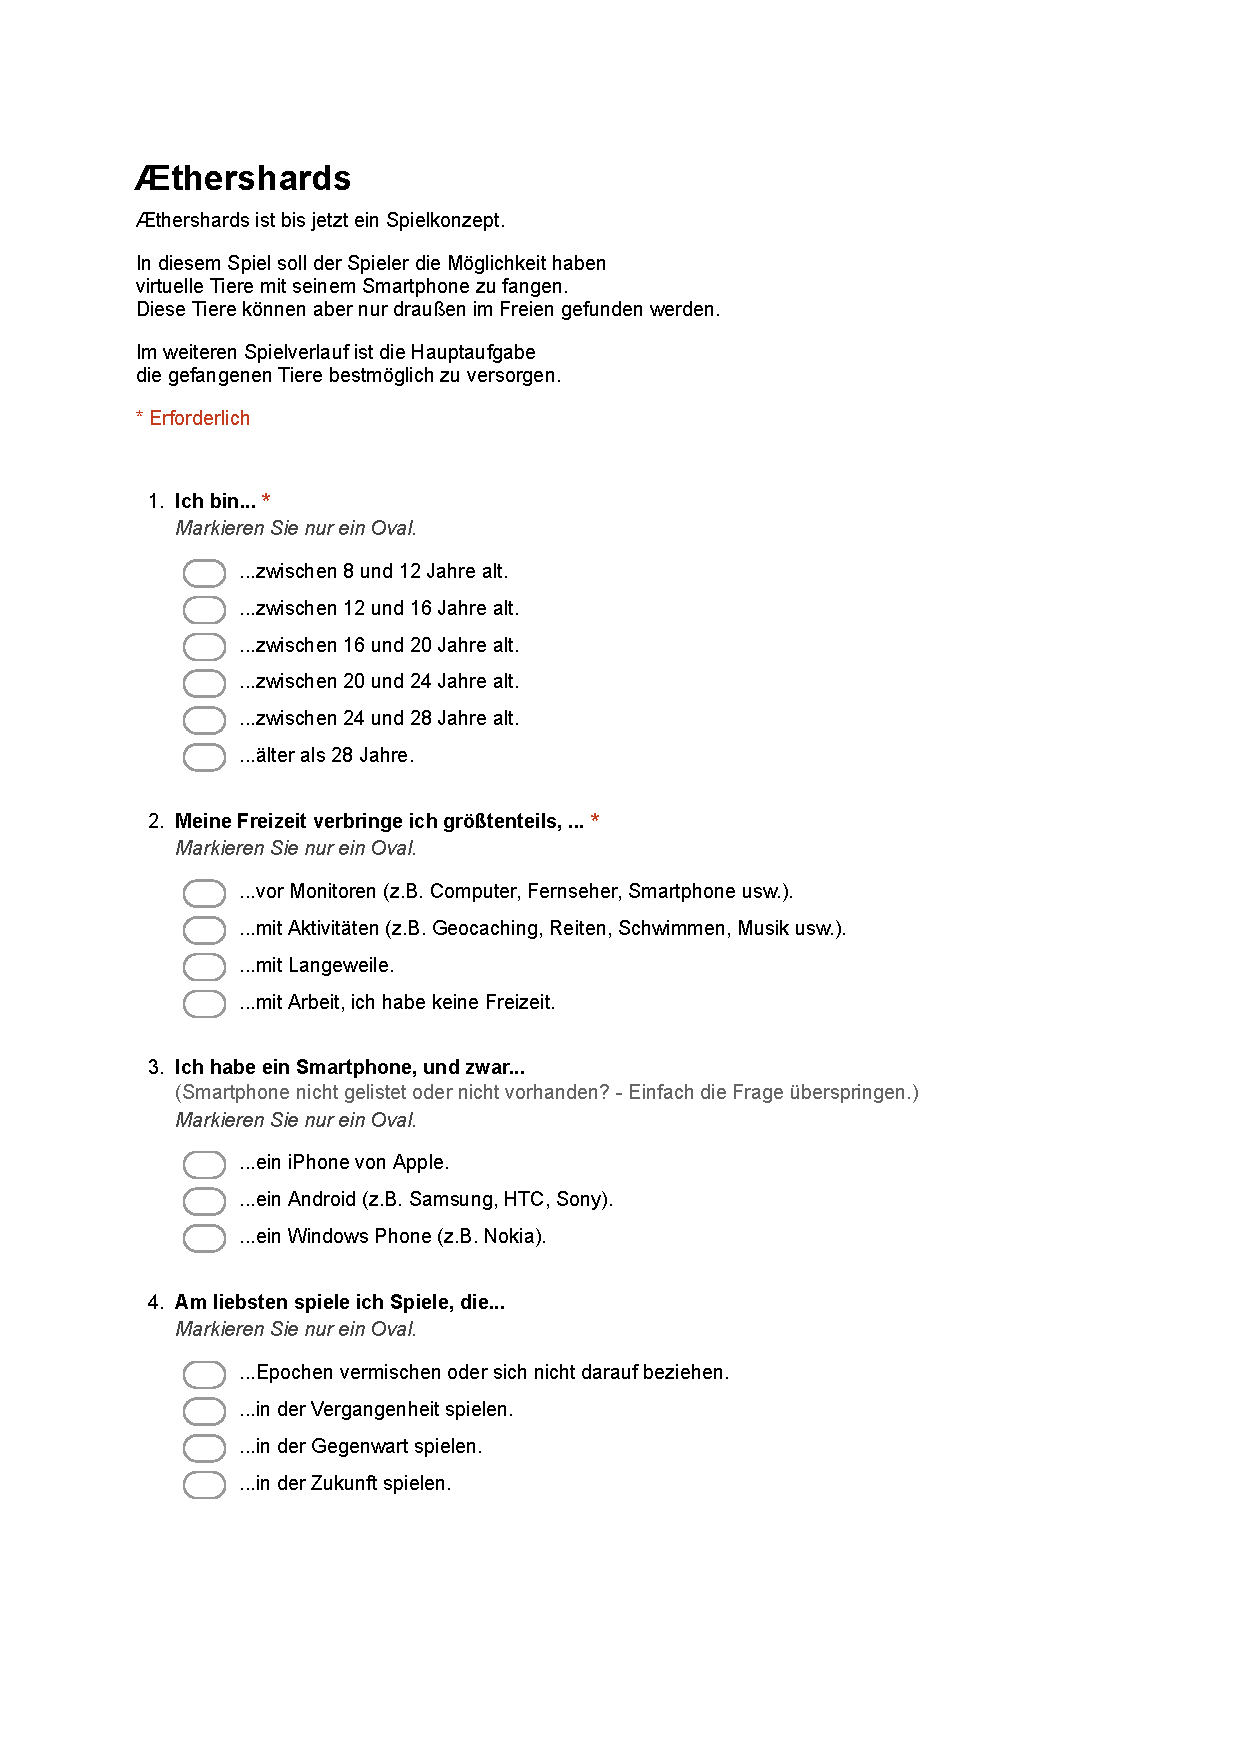
\includepdf[pages={1-3}]{files/umfrage/umfrageclean.pdf}
%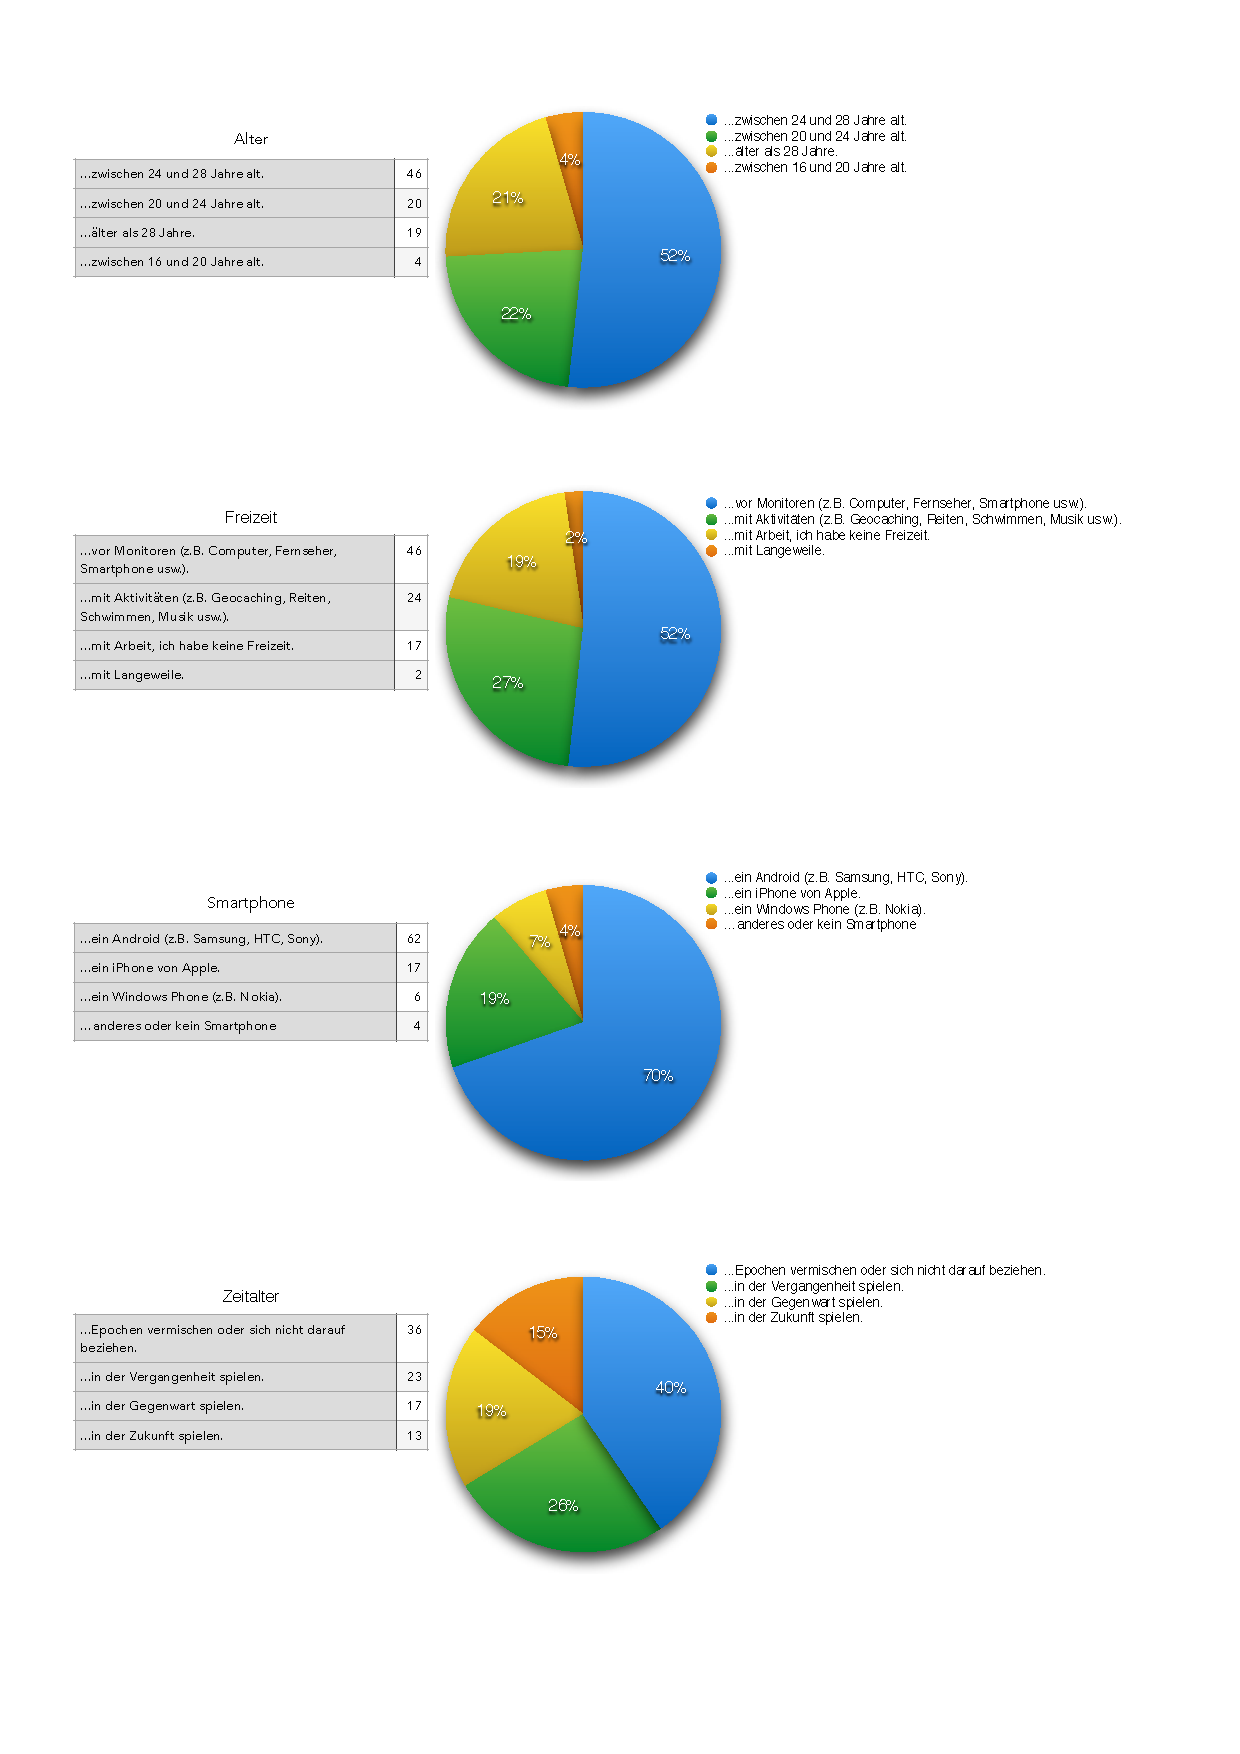
\includepdf[pages={1-3}]{files/umfrage/ergebnisse.pdf}

%\begin{figure}[H]
%    \centering
%    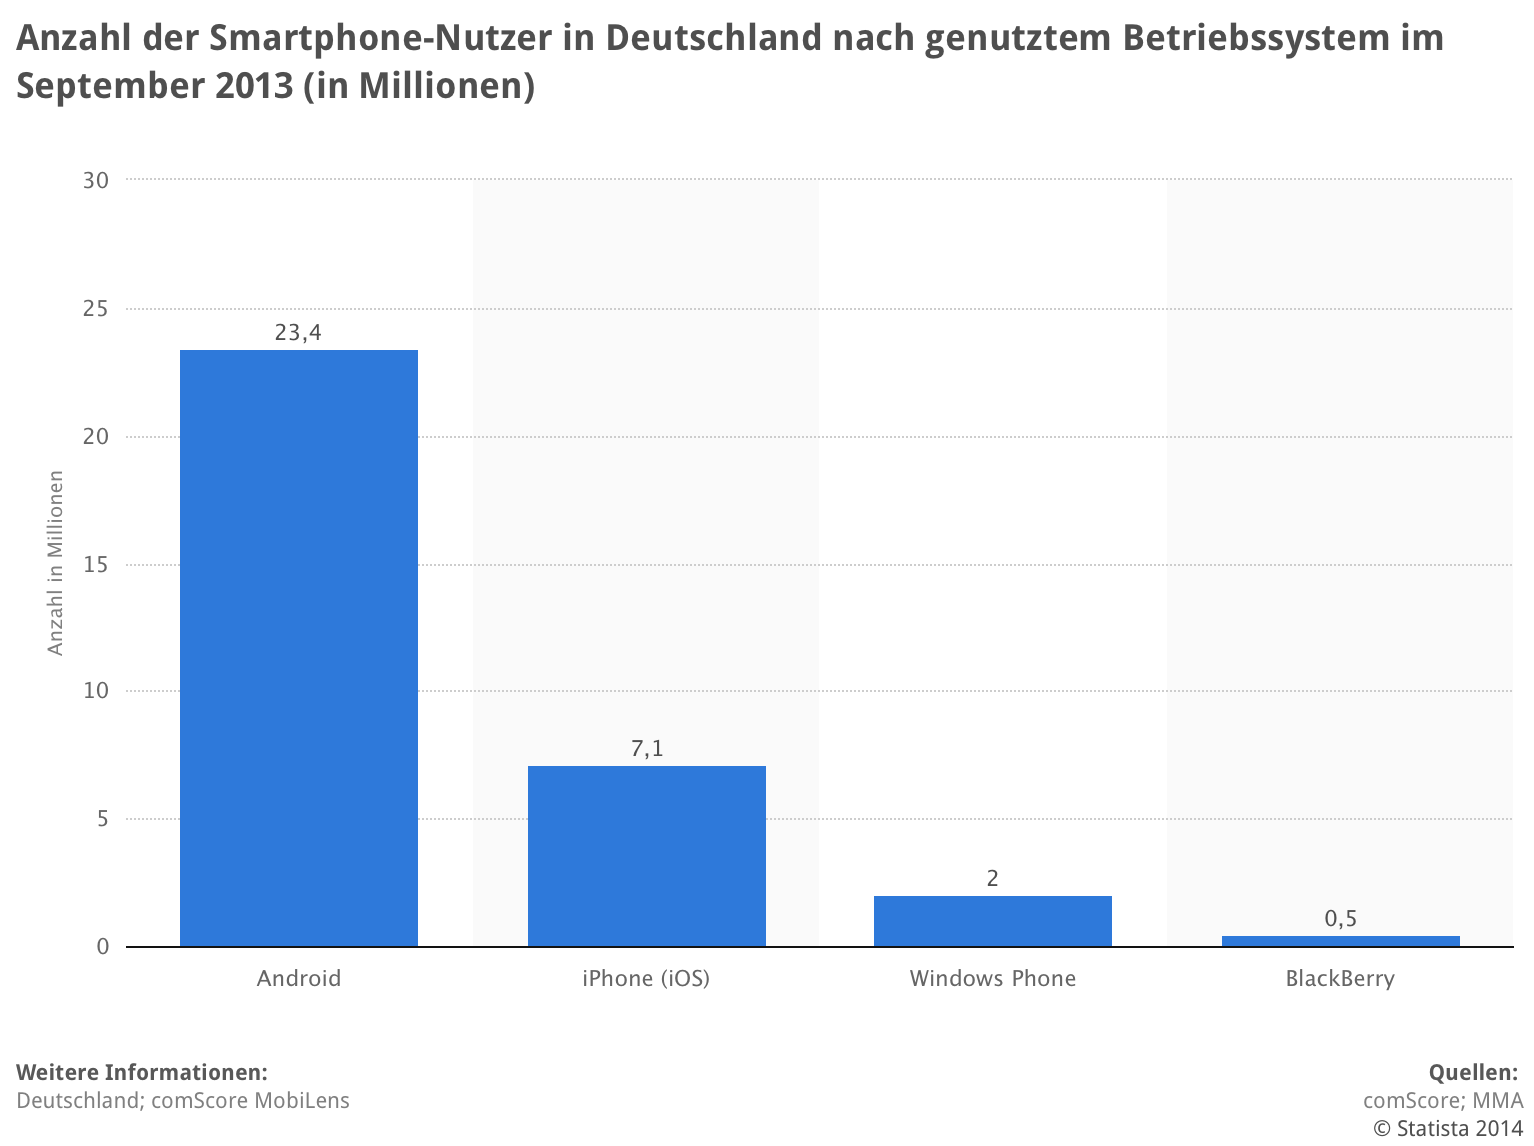
\includegraphics[width=1.01\textwidth]{files/umfrage/smartphoneVerteilung}
%\end{figure}

%\begin{figure}[H]
%    \centering
%    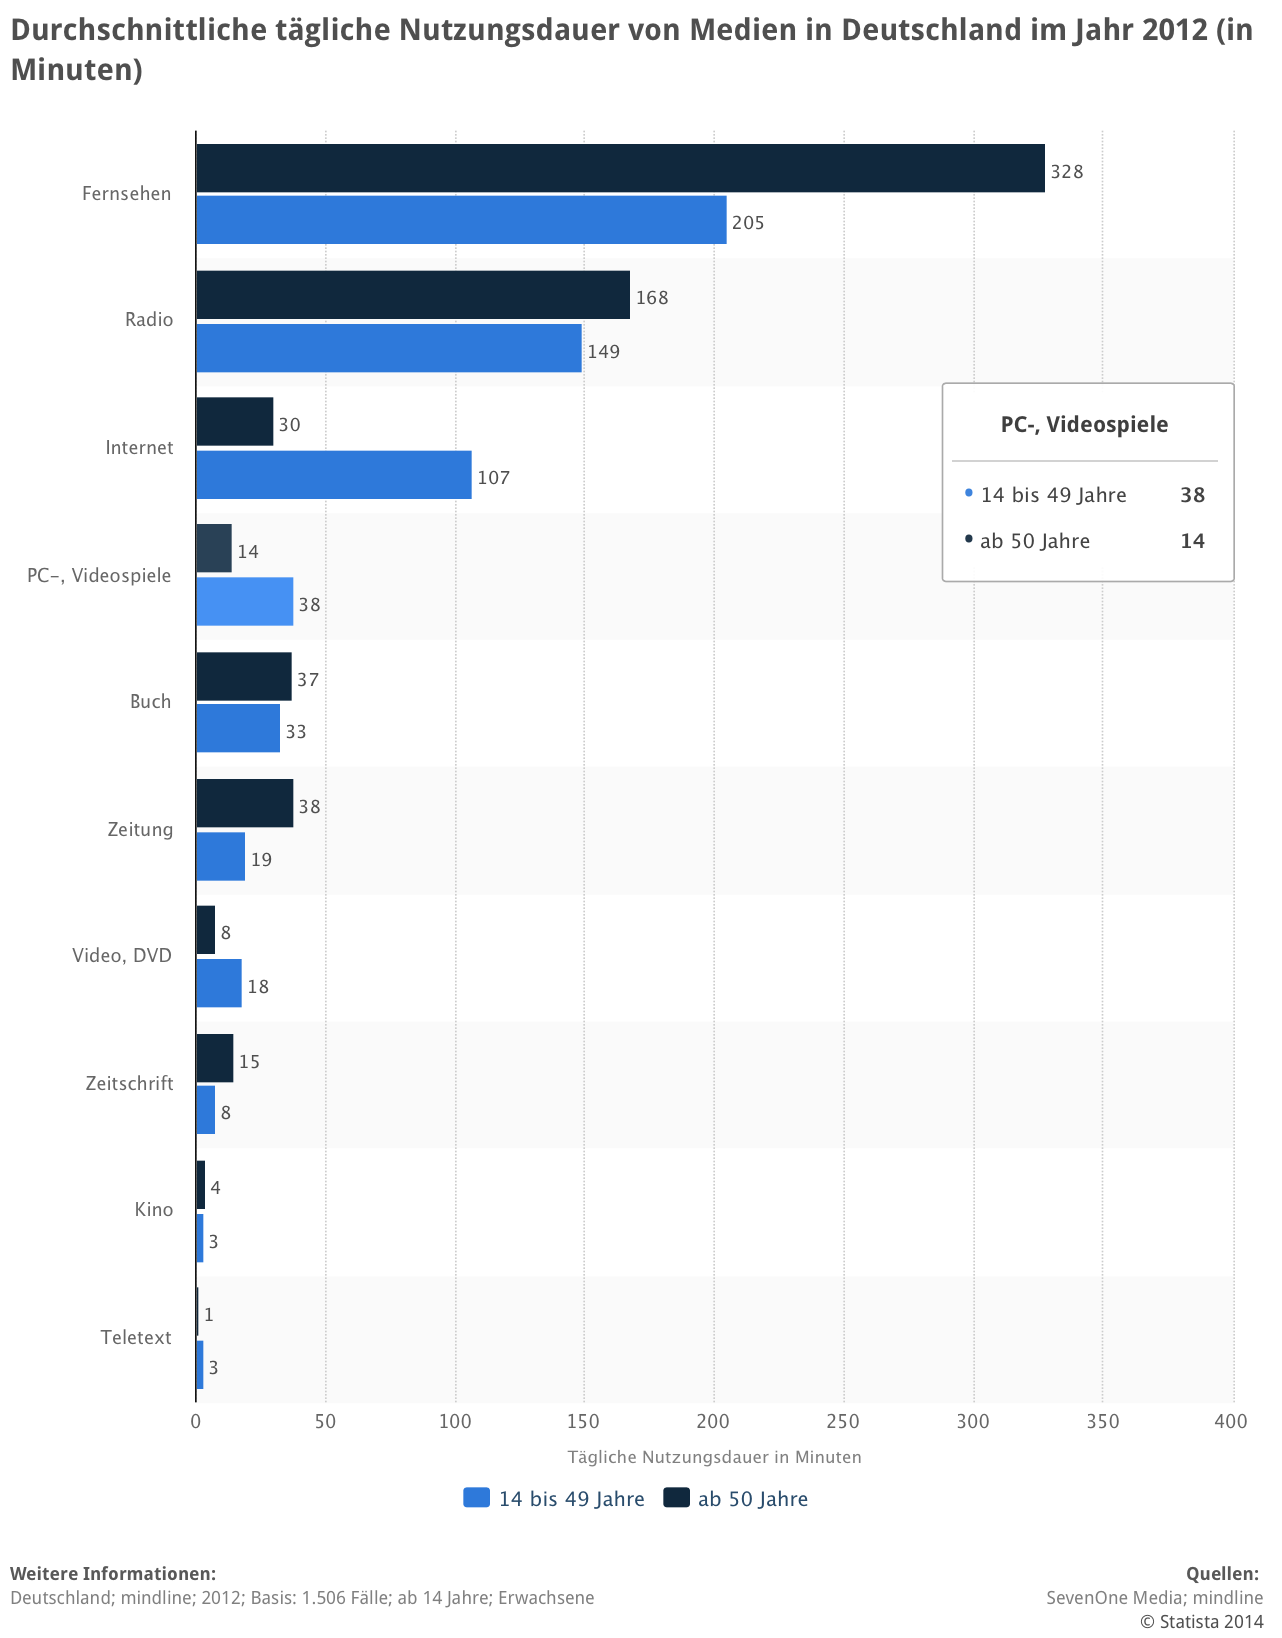
\includegraphics[width=1.01\textwidth]{files/umfrage/medienNutzung}
%\end{figure}
%\textbf{!Zusätzliche Statistiken anhängen!}



\begin{figure}[H]
    \centering
    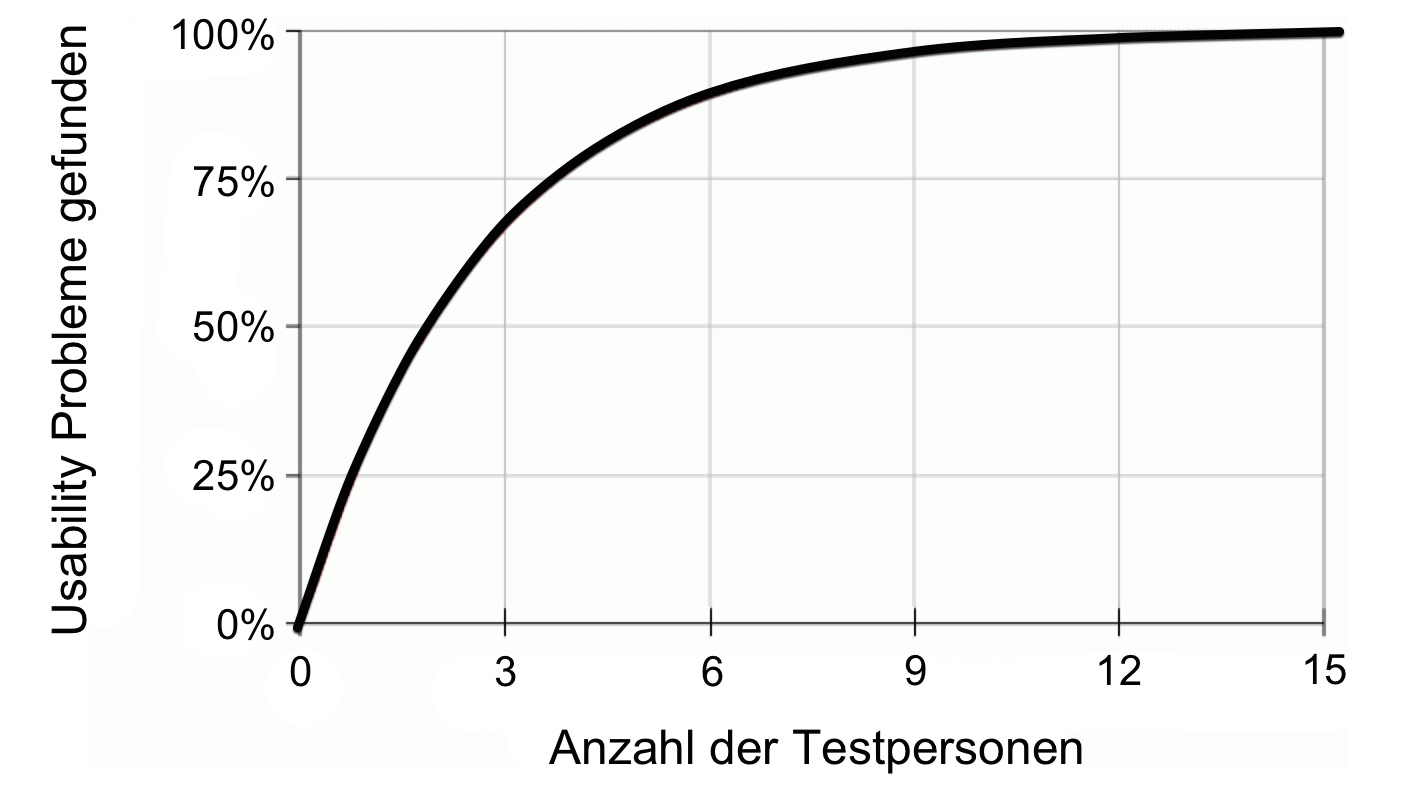
\includegraphics[width=.8\textwidth]{files/usa/anzahlTester}
    \caption{Verhältnis zwischen gefunden Usability Problemen und der Anzahl der Tester vgl. \cite{Nielsen:uc}}
    \label{pic:UsaTesters}
\end{figure}
	%\chapter*{Eidesstattliche Erklärung}
Gemäß §\,17,(5) der BPO erkläre ich an Eides statt, dass ich die vorliegende Arbeit
selbständig angefertigt habe. Ich habe mich keiner fremden Hilfe bedient und keine
anderen, als die angegebenen Quellen und Hilfsmittel benutzt. Alle Stellen, die
wörtlich oder sinngemäß veröffentlichten oder nicht veröffentlichten Schriften und
anderen Quellen entnommen sind, habe ich als solche kenntlich gemacht. Diese
Arbeit hat in gleicher oder ähnlicher Form noch keiner Prüfungsbehörde vorgelegen.
\vspace{3\baselineskip}\\
Dortmund, \thedate \hfill \theauthor

\vspace{1cm}
\section*{Erklärung}
Mir ist bekannt, dass nach §\,156~StGB bzw. §\,163~StGB eine falsche Versicherung
an Eides Statt bzw. eine fahrlässige falsche Versicherung an Eides Statt mit
Freiheitsstrafe bis zu drei Jahren bzw. bis zu einem Jahr oder mit Geldstrafe
bestraft werden kann.
\vspace{3\baselineskip}\\
Dortmund, \thedate \hfill \theauthor

\end{document}
